\addchap{A Anmerkung zur Nutzung von Künstlicher Intelligenz}
\setcounter{chapter}{1}

Im Rahmen dieser Arbeit wurden Künstliche Intelligenz (\acrshort{acr:KI})\index{Künstliche Intelligenz} basierte Werkzeuge benutzt. Tabelle~\ref{tab:anhang_uebersicht_KI_werkzeuge} gibt eine Übersicht über die verwendeten Werkzeuge und den jeweiligen Einsatzzweck.


\begin{table}[hbt]	
	\centering
	\renewcommand{\arraystretch}{1.5}	% Skaliert die Zeilenhöhe der Tabelle
	\captionabove[Liste der verwendeten Künstliche Intelligenz basierten Werkzeuge]{Liste der verwendeten KI basierten Werkzeuge}
	\label{tab:anhang_uebersicht_KI_werkzeuge}
	\begin{tabular}{>{\raggedright\arraybackslash}p{0.3\linewidth} >{\raggedright\arraybackslash}p{0.65\linewidth}}
		\textbf{Werkzeug} & \textbf{Beschreibung der Nutzung}\\
		\hline
		\hline
		ChatGPT & 
		\vspace{-\topsep}
		\begin{itemize}[noitemsep,topsep=0pt,partopsep=0pt,parsep=0pt]
			\item Verständniserklärungen, Rechtschreib- und Grammatikprüfung, Formulierungshilfe, Unterstützung bei Literaturrecherchen, Zusammenfassung wissenschaftlicher Studien und Quellen
		\end{itemize} \\
		Perplexity AI &
		\vspace{-\topsep}
		\begin{itemize}[noitemsep,topsep=0pt,partopsep=0pt,parsep=0pt]
			\item Unterstützung bei Literaturrecherchen(siehe \autoref{cha:Grundlagen})
		\end{itemize} \\
		Claude &
		\vspace{-\topsep}
		\begin{itemize}[noitemsep,topsep=0pt,partopsep=0pt,parsep=0pt]
			\item Unterstützung bei Programmieraufgaben, beim Erstellen von LaTeX-Tabellen, .bib-Dateien oder Diagrammen, sowie bei der Softwareentwicklung in Python.
		\end{itemize} \\
		CoPilot &
		\vspace{-\topsep}
		\begin{itemize}[noitemsep,topsep=0pt,partopsep=0pt,parsep=0pt]
			\item In Visual Studio Code integriert zur automatischen Generierung von Codevorschlägen, zur Unterstützung bei Fehlerbehebungen
		\end{itemize} \\
		Gemini &
		\vspace{-\topsep}
		\begin{itemize}[noitemsep,topsep=0pt,partopsep=0pt,parsep=0pt]
			\item Rechtschreib- \& Grammatikprüfung, Formulierungshilfe
		\end{itemize} \\
		DeepL &
		\vspace{-\topsep}
		\begin{itemize}[noitemsep,topsep=0pt,partopsep=0pt,parsep=0pt]
			\item Übersetzung fremdsprachiger Quellen
		\end{itemize} \\
		\hline
		
	\end{tabular} 
\end{table}
\addchap{B Autorenverzeichnis}
\setcounter{chapter}{2}

\begin{table}[h]
	\centering
	\caption{Autorenverzeichnis der Kapitelzuordnung}
	\label{tab:autorenverzeichnis1}
	\renewcommand{\arraystretch}{1.5}
	
	\begin{tabular}{p{10cm} l}
		\toprule
		\textbf{Kapitel} & \textbf{Autor} \\
		\midrule
		Kurzfassung & Faik Hadutoglu \\
		
		\hyperref[cha:Einleitung]{1. Einleitung} 
		& Faik Hadutoglu \\
		
		\hyperref[cha:Mechatronische Systeme]{2.1 Mechatronische Systeme} 
		& Simon Steiger \\
		
		\hyperref[cha:Definition und Systemarchitektur]{2.1.1. Definition und Systemarchitektur} 
		& Vorname Nachname \\
		
		\hyperref[cha:Interdisziplinäre Integration]{2.1.2. Interdisziplinäre Integration} 
		& Vorname Nachname \\
		
		\hyperref[cha:Elektrische Antriebstechnik]{2.2. Elektrische Antriebstechnik} 
		& Simon Steiger \\
		
		\hyperref[cha:Funktionsweise von Elektromotoren (DC)]{2.2.1. Funktionsweise von Elektromotoren (DC)} 
		& Simon Steiger \\
		
		\hyperref[cha:BDC- und BLDC-Motoren: Grundlagen und Unterschiede]{2.3. BDC- und BLDC-Motoren: Grundlagen und Unterschiede} 
		& Simon Steiger \\
		
		\hyperref[cha:Servomotoren]{2.3.1. Servomotoren} 
		& Simon Steiger \\
		
		\hyperref[cha:Hoverboard-Motoren]{2.3.2. Hoverboard-Motoren} 
		& Simon Steiger \\
		
		\hyperref[cha:Motortreiber und PWM-Steuerung]{2.3.3. Motortreiber und PWM-Steuerung} 
		& Angus Bach \\
		
		\hyperref[cha:Mikrocontroller und Steuerungseinheiten]{2.4. Mikrocontroller und Steuerungseinheiten} 
		& Faik Hadutoglu \\
		
		\hyperref[cha:ESP32]{2.4.1. ESP32} 
		& Faik Hadutoglu \\
		
		\hyperref[cha:Einplatinencomputer und Raspberry Pi]{2.4.2. Einplatinencomputer und Raspberry Pi} 
		& Simon Steiger \\
		
		%\hyperref[cha:Einleitung]{Kapitel} & Vorname Nachname \\
		
		& \\
		
		& \\
		
		& Fortsetzung auf nächster Seite \\
		
		%\bottomrule
	\end{tabular}
\end{table}

\newpage
\begin{table}[h]
	\centering
	\label{tab:autorenverzeichnis2}
	\renewcommand{\arraystretch}{1.5}
	
	\begin{tabular}{p{10cm} l}
		\hyperref[cha:Energieversorgung]{2.5. Energieversorgung} 
		& Faik Hadutoglu \\
		
		\hyperref[cha:Batterie]{2.5.1. Batterie} 
		& Faik Hadutoglu \\
		
		\hyperref[cha:Spannungswandler und Stromverteilung]{2.5.2. Spannungswandler und Stromverteilung} 
		& Angus Bach \\
		
		\hyperref[cha:Additive Fertigungsverfahren (3D-Druck)]{2.6. Additive Fertigungsverfahren (3D-Druck)} 
		& Angus Bach \\
		
		\hyperref[cha:Human-Machine-Interaction]{2.7. Human-Machine-Interaction} 
		& Hai Nam Nguyen \\
		
		\hyperref[cha:Definitionen und Zielsetzung]{2.7.1. Definitionen und Zielsetzung} 
		& Hai Nam Nguyen \\
		
		\hyperref[cha:Interaktionsformen]{2.7.2. Interaktionsformen} 
		& Hai Nam Nguyen \\
		
		\hyperref[cha:Nutzerzentriertes Design]{2.7.3. Nutzerzentriertes Design} 
		& Hai Nam Nguyen \\
		
		\hyperref[cha:Visualisierung und Interaktionssystem]{2.7.4. Visualisierung und Interaktionssystem} 
		& Hai Nam Nguyen \\
		
		%\hyperref[cha:Projekt und Systems Engineering Methodik]{2.8. Projekt \& Systems Engineering Methodik} & Vorname Nachname \\
		
		\hyperref[cha:Scrum]{2.8.1. Scrum} 
		& Angus Bach \\
		
		\hyperref[cha:V-Modell]{2.8.2. V-Modell} 
		& Angus Bach \\
		
		\hyperref[cha:SWOT-Analyse]{2.8.3. SWOT-Analyse} 
		& Hai Nam Nguyen \\
		
		\hyperref[cha:Gantt-Diagramm]{2.8.4. Gantt-Diagramm} 
		& Hai Nam Nguyen \\
		
		%\hyperref[cha:Einleitung]{Kapitel} & Vorname Nachname \\
		
		& \\
		
		& \\
		
		& Fortsetzung auf nächster Seite \\
		
		%\bottomrule
	\end{tabular}
\end{table}

\newpage
\begin{table}[h]
	\centering
	\label{tab:autorenverzeichnis3}
	\renewcommand{\arraystretch}{1.5}
	
	\begin{tabular}{p{10cm} l}
		\hyperref[cha:Projektorganisation]{3.1. Projektorganisation} & Angus Bach \\
		
		\hyperref[cha:Anforderungsanalyse]{3.2. Anforderungsanalyse} & Angus Bach \\
		
		\hyperref[cha:Designkonzept]{3.3. Designkonzept} & Angus Bach \\
		
		\hyperref[cha:Vergleich: Räder vs. Ketten]{3.3.1. Vergleich: Räder vs. Ketten} & Angus Bach \\
		
		\hyperref[cha:Entscheidungsfindung und Begründung]{3.3.2. Entscheidungsfindung und Begründung} & Angus Bach \\
		
		\hyperref[cha:Steuerungskonzept]{3.4. Steuerungskonzept} & Faik Hadutoglu \\
		
		\hyperref[cha:Grundlegende Signalverarbeitung]{3.4.1. Grundlegende Signalverarbeitung} & Faik Hadutoglu \\
		
		\hyperref[cha:Differenzielle Bewegungssteuerung]{3.4.2. Differenzielle Bewegungssteuerung} & Faik Hadutoglu \\
		
		\hyperref[cha:Begrenzung und Schutzmechanismen]{3.4.3. Begrenzung und Schutzmechanismen} & Faik Hadutoglu \\
		
		\hyperref[cha:Ablaufbasierte Steuerungslogik]{3.4.4. Ablaufbasierte Steuerungslogik} & Faik Hadutoglu \\
		
		\hyperref[cha:Interaktionsdesign]{3.5. Interaktionsdesign} & Vorname Nachname \\
		
		\hyperref[cha:Display-Integration]{3.5.1. Display-Integration} & Vorname Nachname \\
		
		\hyperref[cha:Augen-Animation und Emotionsdarstellung]{3.5.2. Augen-Animation und Emotionsdarstellung} & Angus Bach \\
		
		\hyperref[cha:Benutzerinteraktion]{3.5.3. Benutzerinteraktion} & Hai Nam Nguyen \\
		
		\hyperref[cha:Systemarchitektur]{3.6. Systemarchitektur} & Vorname Nachname \\
		
		\hyperref[cha:Komponentenauswahl]{3.6.1. Komponentenauswahl} & Vorname Nachname \\
		
		\hyperref[cha:Elektronische Architektur]{3.6.2. Elektronische Architektur} & Angus Bach \\
		
		\hyperref[cha:Einleitung]{3.6.3. Umsetzungsmöglichkeiten innerhalb der Praxisphase } & Hai Nam Nguyen \\
		
		\hyperref[cha:Projektplanung und Meilensteine]{3.7. Projektplanung und Meilensteine} & Hai Nam Nguyen \\
		
		\hyperref[cha:Aufteilung der Arbeitspakete]{3.7.1. Aufteilung der Arbeitspakete} & Faik Hadutoglu \\
		
		\hyperref[cha:Definition von Meilensteinen]{3.7.2. Definition von Meilensteinen} & Faik Hadutoglu \\
		
		\hyperref[cha:Budgetplanung]{3.8.1. Budgetplanung} & Angus Bach \\
		
		\hyperref[cha:Aktuelle Kostenschätzung]{3.8.2. Aktuelle Kostenschätzung} & Hai Nam Nguyen \\
		
		\hyperref[cha:Bewertung des Projekts]{3.9. Bewertung des Projekts} & Hai Nam Nguyen \\
		
		\hyperref[cha:SWOT-Analyse des Messe-Roboters]{3.9.1. SWOT-Analyse des Messe-Roboters} & Hai Nam Nguyen \\
		
		\hyperref[cha:SWOT-Analyse des Projekts aus Sicht der Hochschule]{3.9.2. SWOT-Analyse des Projekts aus Sicht der Hochschule} & Hai Nam Nguyen \\
		
		\hyperref[cha:Finale Bewertung]{3.9.3. Finale Bewertung} & Hai Nam Nguyen \\
		
		%\hyperref[cha:Einleitung]{Kapitel} & Vorname Nachname \\
		
		& \\
		
		& \\
		
		& Fortsetzung auf nächster Seite \\
		
		%\bottomrule
	\end{tabular}
\end{table}

\newpage
\begin{table}[h]
	\centering
	\label{tab:autorenverzeichnis4}
	\renewcommand{\arraystretch}{1.5}
	
	\begin{tabular}{p{10cm} l}
		\hyperref[cha:CAD-Modellierung]{4.1.1. CAD-Modellierung} & Vorname Nachname \\
		
		\hyperref[cha:Montage und Nachbearbeitung]{4.1.2. Montage und Nachbearbeitung} & Vorname Nachname \\
		
		\hyperref[cha:Motorsteuerung und Bewegungsalgorithmen]{4.2. Motorsteuerung und Bewegungsalgorithmen} & Faik Hadutoglu \\
		
		\hyperref[cha:Fernsteuerungssystem und Signalübertragung]{4.2.1. Fernsteuerungssystem und Signalübertragung} & Vorname Nachname \\
		
		\hyperref[cha:Programmablauf und Architektur]{4.2.2. Programmablauf und Architektur} & Faik Hadutoglu \\
		
		\hyperref[cha:Detaillierte Implementierung]{4.2.3. Detaillierte Implementierung} & Faik Hadutoglu \\
		
		\hyperref[cha:Display-Programmierung]{4.3. Display-Programmierung} & Simon Steiger \\
		
		\hyperref[cha:Animations-Engine für Augen]{4.3.1. Animations-Engine für Augen} & Simon Steiger \\
		
		\hyperref[cha:Benutzerschnittstelle]{4.3.2. Benutzerschnittstelle} & Simon Steiger \\
		
		\hyperref[cha:Integrationsstrategie]{4.4.1. Integrationsstrategie} & Angus Bach \\
		
		\hyperref[cha:Subsystemtests des Fahr- und Antriebssystems]{4.4.2. Subsystemtests des Fahr- und Antriebssystems} & Angus Bach \\
		
		\hyperref[cha:Subsystemtests der Augenansteurung über Display und Kamera]{4.4.3. Subsystemtests der Augenansteurung über Display und Kamera} & Simon Steiger \\
		
		\hyperref[cha:Implementierung eines Failsafe-Mechanismus]{4.4.4. Implementierung eines Failsafe-Mechanismus} & Faik Hadutoglu \\
		
		\hyperref[cha:Ergebnisse und Diskussion]{5. Ergebnisse und Diskussion} & Faik Hadutoglu \\
		
		
		\hyperref[cha:Zusammenfassung und Fazit]{6. Zusammenfassung und Fazit} & Faik Hadutoglu \\
	
		%\hyperref[cha:Einleitung]{Kapitel} & Vorname Nachname \\
		
		\bottomrule
	\end{tabular}
\end{table}
\clearpage

%\chapter{Schaltpläne}
\chapter{Stückliste und Kostenkalkulation}
\label{sec:Stückliste}
\begin{longtable}{|p{4cm}|p{7cm}|p{2.5cm}|}
	\hline
	\textbf{Artikel} & \textbf{Beschreibung/Link} & \textbf{Preis* (€)} \\
	\hline
	\endfirsthead
	
	\hline
	\textbf{Artikel} & \textbf{Beschreibung/Link} & \textbf{Preis (€)} \\
	\hline
	\endhead
	
	Vorders Freirad & \url{https://amzn.eu/d/2R2QoEb} & 10.10 \\
	\hline
	
	Motor & \url{https://amzn.eu/d/31wBcL6} & 29.00 \\
	\hline
	
	Motor Treiber / Regler & \url{https://amzn.eu/d/hQnLU2L} & 23.00 \\
	\hline
	
	2× Arme & X & \\
	\hline
	
	Kamera & https://amzn.eu/d/c3tmM8x & 78.45 \\
	\hline
	
	Raspberry Pi 5 & RASPBERRY PI Raspberry Pi 5 B, 4x 2,4 GHz, 8 GB RAM, WLAN/BT \newline \url{https://www.reichelt.de/de/de/shop/produkt/raspberry_pi_5_b_4x_2_4_ghz_8_gb_ram_wlan_bt-359846} & 84.50 \\
	\hline
	
	ESP32 & 3 STK \newline ESP32 Dev Kit C V4 unverlötet kompatibel mit Arduino \newline \url{https://www.az-delivery.de/products/esp32-dev-kit-c-v4-unverlötet?variant=32437206614112} & 23.99 \\
	\hline
	
	SD Karte & \url{https://t1p.de/0a2o2} & 29.99 \\
	\hline
	
	DC/DC & 1 Stck: BGTXINGI XL4016E1 Hochleistungs DC Druckregulierung Konstantstromregler Konverter für Laden oder LED-Treibermodul \newline \url{https://amzn.eu/d/4Ip4AZM} & 10.99 \\
	\hline
	
	Schutztasche & 1 STK: \url{https://amzn.eu/d/4HDhlFv} & 9.99 \\
	\hline
	
	Ladegerät/Lipo-Akku & 1 STK: Spektrum Smart G2 S155 AC Ladegerät 1x55W (EU Version) \newline \url{https://url-shortener.me/6W9W} & 62.95 \\
	\hline
	
	Servomotoren für Kopf & 2 Stk: \url{https://amzn.eu/d/c8CYSqc} & 24.98 \\
	\hline
	
	Lautsprecher & 1 Stk: ADELGO SoundBar Mini USB Lautsprecher \newline \url{https://amzn.eu/d/7B3o9JZ} & 18.99 \\
	\hline
	
	Display & 1 stk: \url{https://amzn.eu/d/iOJQEvv} & 62.99 \\
	\hline
	
	Sprühdosen & X & \\
	\hline
	
	Raspberry Pi 5 Kühler & \url{https://amzn.eu/d} & 9.99 \\
	\hline
	
	Powerbank & \url{https://amzn.eu/d/dUgwX30} & 35.99 \\
	\hline
	
	Spannungsprüfer & \url{https://amzn.eu/d/ejeywWj} & 5.99 \\
	\hline
	
	Rad & 4 Stk: \url{https://amzn.eu/d/d5vTwyP} \newline Zur Not: \url{https://amzn.eu/d/fWLkApq} & 19.59 $\times$ 4 \\
	\hline
	
	\multicolumn{2}{|r|}{\textbf{Total (Ohne Lieferungsgebühren)}} & \textbf{600,25} \\
	\hline
	
\end{longtable}

* Alle in dieser Hausarbeit aufgeführten Preisangaben wurden zum Zeitpunkt der Bearbeitung recherchiert. Änderungen der Preise nach diesem Zeitpunkt sind möglich.




\chapter{Quellcode (Auszüge)}

%\begin{lstlisting}[style=motorStyle, caption={Begrenzung der Ausgangsspannung}]
%	
%\end{lstlisting}

\section{Motorsteuerung}

\begin{lstlisting}[style=motorStyle, caption={Motorsteuerung: acutatorController.cpp}]

//acutatorController.cpp
#include "actuatorController.h"

/******************************************************************************
* Private Declarations
******************************************************************************/
#define AUTOPILOT_LED_BLINK_RATE_AVAILABLE_AND_ACTIVATED 25
#define AUTOPILOT_LED_BLINK_RATE_AVAILABLE 5
#define AUTOPILOT_LED_BLINK_RATE_AUOTOPILOT_OFF 5000

#define ELEVATOR 0
#define AILERON 1
#define RUDDER 2
#define ENGINE 3
#define FLAP 4
#define NUMBER_OF_SERVOS 5 //Elevator,Aileron,Rudder,Engine,Flap

#define MINIMUM_ANGLE_SERVO 0
#define MAXIMUM_ANGLE_SERVO 180
#define MINIMUM_VALID_PULSE_LENGTH_SERVO 1000
#define MAXIMUM_VALID_PULSE_LENGTH_SERVO 2000

#define FLAP_NEUTRAL_POSITION_PULSE_LENGTH_US 1091

/******************************************************************************
* Private Variables
******************************************************************************/
static bool moduleIsInitialised = false;

static Servo servo[NUMBER_OF_SERVOS];
static uint8_t servoSignalPinsESP[NUMBER_OF_SERVOS] = {PIN_ELEVATOR_RECEIVED_ESP, PIN_AILERON_RECEIVED_ESP, PIN_RUDDER_RECEIVED_ESP, PIN_SPEED_RECEIVED_ESP, PIN_FLAP_RECEIVED_ESP};
static uint8_t servoSignalPinsRC[NUMBER_OF_SERVOS] = {PIN_ELEVATOR_RECEIVED_RC, PIN_AILERON_RECEIVED_RC, PIN_RUDDER_RECEIVED_RC, PIN_SPEED_RECEIVED_RC, PIN_FLAP_RECEIVED_RC};

/******************************************************************************
* Public Functions
******************************************************************************/
void actuatorControllerInit(){
	// To read PWM Signals from ESP32/Autopilot
	// pinMode(PIN_ELEVATOR_RECEIVED_ESP, INPUT);
	// pinMode(PIN_SPEED_RECEIVED_ESP, INPUT);
	// pinMode(PIN_AILERON_RECEIVED_ESP, INPUT);
	// pinMode(PIN_RUDDER_RECEIVED_ESP, INPUT);
	// pinMode(PIN_FLAP_RECEIVED_ESP, INPUT); // Currently not used
	
	
	
	
	// EXPODROID PWM-Pins konfigurieren
	//Module 1 
	pinMode(PIN_BTS1_RPWM, OUTPUT);
	pinMode(PIN_BTS1_LPWM, OUTPUT);
	//Modul2
	pinMode(PIN_BTS2_RPWM, OUTPUT);
	pinMode(PIN_BTS2_LPWM, OUTPUT);
	
	
	
	
	// To read PWM Signals from Remote Control
	pinMode(PIN_ELEVATOR_RECEIVED_RC, INPUT);
	pinMode(PIN_SPEED_RECEIVED_RC, INPUT);
	pinMode(PIN_AILERON_RECEIVED_RC, INPUT);
	pinMode(PIN_RUDDER_RECEIVED_RC, INPUT);
	pinMode(PIN_FLAP_RECEIVED_RC, INPUT);
	
	// To write PWM signals to servos
	servo[ELEVATOR].attach(PIN_ELEVATOR_CONTROLLER);
	servo[AILERON].attach(PIN_AILERON_CONTROLLER);
	servo[RUDDER].attach(PIN_RUDDER_CONTROLLER);
	servo[ENGINE].attach(PIN_SPEED_CONTROLLER);
	servo[FLAP].attach(PIN_FLAP_CONTROLLER);
	
	pinMode(PIN_AUTOPILOT_LED, OUTPUT);
	
	moduleIsInitialised = true;
}

void actuatorControllerForwardSignals(){
	static uint32_t cnt = 0;
	static uint8_t autopilotLEDState = 0;
	static uint32_t autopilotLEDCounter = 0;
	uint16_t pulseLength_us = 0;
	uint8_t autopilotState = flightguidanceCommunicatorGetAutopilotState();
	
	// EXPODROID: Variablen für Motor-Steuerung
	static int lastSteeringPulse = 1500;
	static int lastSpeedPulse = 1500;
	
	autopilotLEDCounter++;
	
	if(autopilotState == AUTOPILOT_COMMUNICATOR_AUTOPILOT_AVAILABLE && autopilotLEDCounter >= AUTOPILOT_LED_BLINK_RATE_AVAILABLE){ //if autopilot is available
		autopilotLEDState ^= 1;
		digitalWrite(PIN_AUTOPILOT_LED,autopilotLEDState); //LED TOGGLES
		autopilotLEDCounter = 0;
	}
	else if(autopilotState == AUTOPILOT_COMMUNICATOR_AUTOPILOT_AVAILABLE_AND_ACTIVATED){ //if Autopilot is controlling
		digitalWrite(PIN_AUTOPILOT_LED,HIGH); //LED ON
	}
	else if(autopilotState == AUTOPILOT_COMMUNICATOR_AUTOPILOT_NOT_AVAILABLE){ //if autopilot was never enabled, or has a major error 
		digitalWrite(PIN_AUTOPILOT_LED,LOW); //LED OFF
	}
	
	for(int i = 0; i < NUMBER_OF_SERVOS-1; i++){ //Flap must be handled separately, because flight guidance does not send flap servo signals to flight control
		if(autopilotState == AUTOPILOT_COMMUNICATOR_AUTOPILOT_AVAILABLE_AND_ACTIVATED) pulseLength_us = pulseIn(servoSignalPinsESP[i], HIGH, TIMEOUT_SERVO_SIGNAL_HIGH_US ); // if Timeout is exceeded, 0 gets returned -> 0 is NOT the correct pulse Length
		else pulseLength_us = pulseIn(servoSignalPinsRC[i], HIGH, TIMEOUT_SERVO_SIGNAL_HIGH_US );
		if(pulseLength_us != 0){ 
			#ifdef DEBUG_CURRENT_SERVO_ANGLES
			#define PRINT_COUNTS 10
			if(cnt>PRINT_COUNTS){
				switch(i){
					case 0: 
					Serial.println("ELE:"+String(pulseLength_us)+",");
					break;
					case 1: 
					Serial.println("AIL:"+String(pulseLength_us)+",");
					break;
					case 2: 
					Serial.println("RDR:"+String(pulseLength_us)+",");
					break;
					case 3: 
					Serial.println("ENG:"+String(pulseLength_us)+",");
					break;     
				}
			}
			#endif
			
			// EXPODROID: Werte für Motor-Steuerung speichern (wir wollen dc Motoren ansteuern und keine Servos deswegen die Anpassung)
			if(i == ENGINE){
				lastSteeringPulse = pulseLength_us;
			}
			else if(i == AILERON){
				lastSpeedPulse = pulseLength_us;
			}
			
			// Normale Servos (ELEVATOR, RUDDER) direkt ansteuern signal was vom Sender kommt ohne änderung für Servos
			// ENGINE und AILERON werden später für Motoren verwendet
			if(i != ENGINE && i != AILERON){
				servo[i].writeMicroseconds(pulseLength_us);
			}
		}
	}
	
	// EXPODROID: Motor-Steuerung mit den gesammelten Werten
	// Berechne Basis-Geschwindigkeit (-255 bis +255)
	int baseSpeed = 0;
	if(lastSpeedPulse < 1450) {
		// Rückwärts: 1100-1450 -> -255 bis 0
		baseSpeed = map(lastSpeedPulse, 1100, 1450, -255, 0); //mappen bedeutet wert von einem bereich in einen anderen zu übertragen damit er von Motortreiber verstanden wird
	} else if(lastSpeedPulse > 1550) {
		// Vorwärts: 1550-1900 -> 0 bis 255
		baseSpeed = map(lastSpeedPulse, 1550, 1900, 0, 255);
	} else {
		// Deadzone: 1450-1550 = Stop
		baseSpeed = 0;
	}
	
	// Berechne Lenkung (-100 bis +100)
	int steering = 0;
	if(lastSteeringPulse < 1450) {
		// Links: 1000-1450 -> -100 bis 0
		steering = map(lastSteeringPulse, 1000, 1450, -100, 0);
	} else if(lastSteeringPulse > 1550) {
		// Rechts: 1550-2000 -> 0 bis +100
		steering = map(lastSteeringPulse, 1550, 2000, 0, 100);
	}
	
	// Differential Berechnung
	int leftMotorSpeed = baseSpeed;
	int rightMotorSpeed = baseSpeed;
	
	if(steering > 0) {
		// Rechts drehen: rechter Motor langsamer  //bissle: in der Praxis testen ob die Rädergeschwindigkeitsunterschied zu viel wird!!
		rightMotorSpeed = baseSpeed * (100 - steering) / 100;
	} else if(steering < 0) {
		// Links drehen: linker Motor langsamer
		leftMotorSpeed = baseSpeed * (100 + steering) / 100;
	}
	
	// Begrenzung auf -255 bis +255  
	const float batterie_factor = 0.91; //Begrenzung der Spannung // Spitzenspannung kann trzdem mehr als 12V sein??
	leftMotorSpeed = constrain(leftMotorSpeed, -255 * batterie_factor, 255 * batterie_factor);
	rightMotorSpeed = constrain(rightMotorSpeed, -255 * batterie_factor, 255 * batterie_factor);
	
	// Motor 1 (Links) ansteuern
	if(leftMotorSpeed > 0) {
		analogWrite(PIN_BTS1_RPWM, abs(leftMotorSpeed));
		analogWrite(PIN_BTS1_LPWM, 0);
	} else if(leftMotorSpeed < 0) {
		analogWrite(PIN_BTS1_RPWM, 0);
		analogWrite(PIN_BTS1_LPWM, abs(leftMotorSpeed));
	} else {
		analogWrite(PIN_BTS1_RPWM, 0);
		analogWrite(PIN_BTS1_LPWM, 0);
	}
	
	// Motor 2 (Rechts) ansteuern
	if(rightMotorSpeed > 0) {
		analogWrite(PIN_BTS2_RPWM, abs(rightMotorSpeed));
		analogWrite(PIN_BTS2_LPWM, 0);
	} else if(rightMotorSpeed < 0) {
		analogWrite(PIN_BTS2_RPWM, 0);
		analogWrite(PIN_BTS2_LPWM, abs(rightMotorSpeed));
	} else {
		analogWrite(PIN_BTS2_RPWM, 0);
		analogWrite(PIN_BTS2_LPWM, 0);
	}
	
	// Debug-Ausgabe für Motor-Steuerung (immer aktiv für Testen)
	Serial.print("AIL:"); Serial.print(lastSpeedPulse);
	Serial.print(" ENG:"); Serial.print(lastSteeringPulse);
	Serial.print(" Base:"); Serial.print(baseSpeed);
	Serial.print(" Steer:"); Serial.print(steering);
	Serial.print(" L:"); Serial.print(leftMotorSpeed);
	Serial.print(" R:"); Serial.println(rightMotorSpeed);
	
	#ifdef DEBUG_CURRENT_SERVO_ANGLES
	if(cnt++>PRINT_COUNTS){
		cnt = 0;
		Serial.println("");
	} 
	#endif
	
	if(autopilotState == AUTOPILOT_COMMUNICATOR_AUTOPILOT_AVAILABLE_AND_ACTIVATED){
		servo[FLAP].writeMicroseconds(FLAP_NEUTRAL_POSITION_PULSE_LENGTH_US);
	}
	else{
		pulseLength_us = pulseIn(servoSignalPinsRC[FLAP], HIGH, TIMEOUT_SERVO_SIGNAL_HIGH_US);
		servo[FLAP].writeMicroseconds(pulseLength_us);
	}
}


\end{lstlisting}


\begin{lstlisting}[style=motorStyle, caption={Motorsteuerung: main.cpp}]
	
	//main.cpp
	#include "actuatorController.h"
	#include <Arduino.h>
	#include "actuatorController.h"
	#include "flightguidanceCommunicator.h"
	...
	...
	// ================================================================
	// ===                    MAIN PROGRAM LOOP                     ===
	// ================================================================
	
	void loop()
	{
		actuatorControllerForwardSignals();
	}
	
\end{lstlisting}


%\chapter{Technische Zeichnungen}
\chapter{Datenblätter / Herstellerdokumentation wichtiger Komponenten}

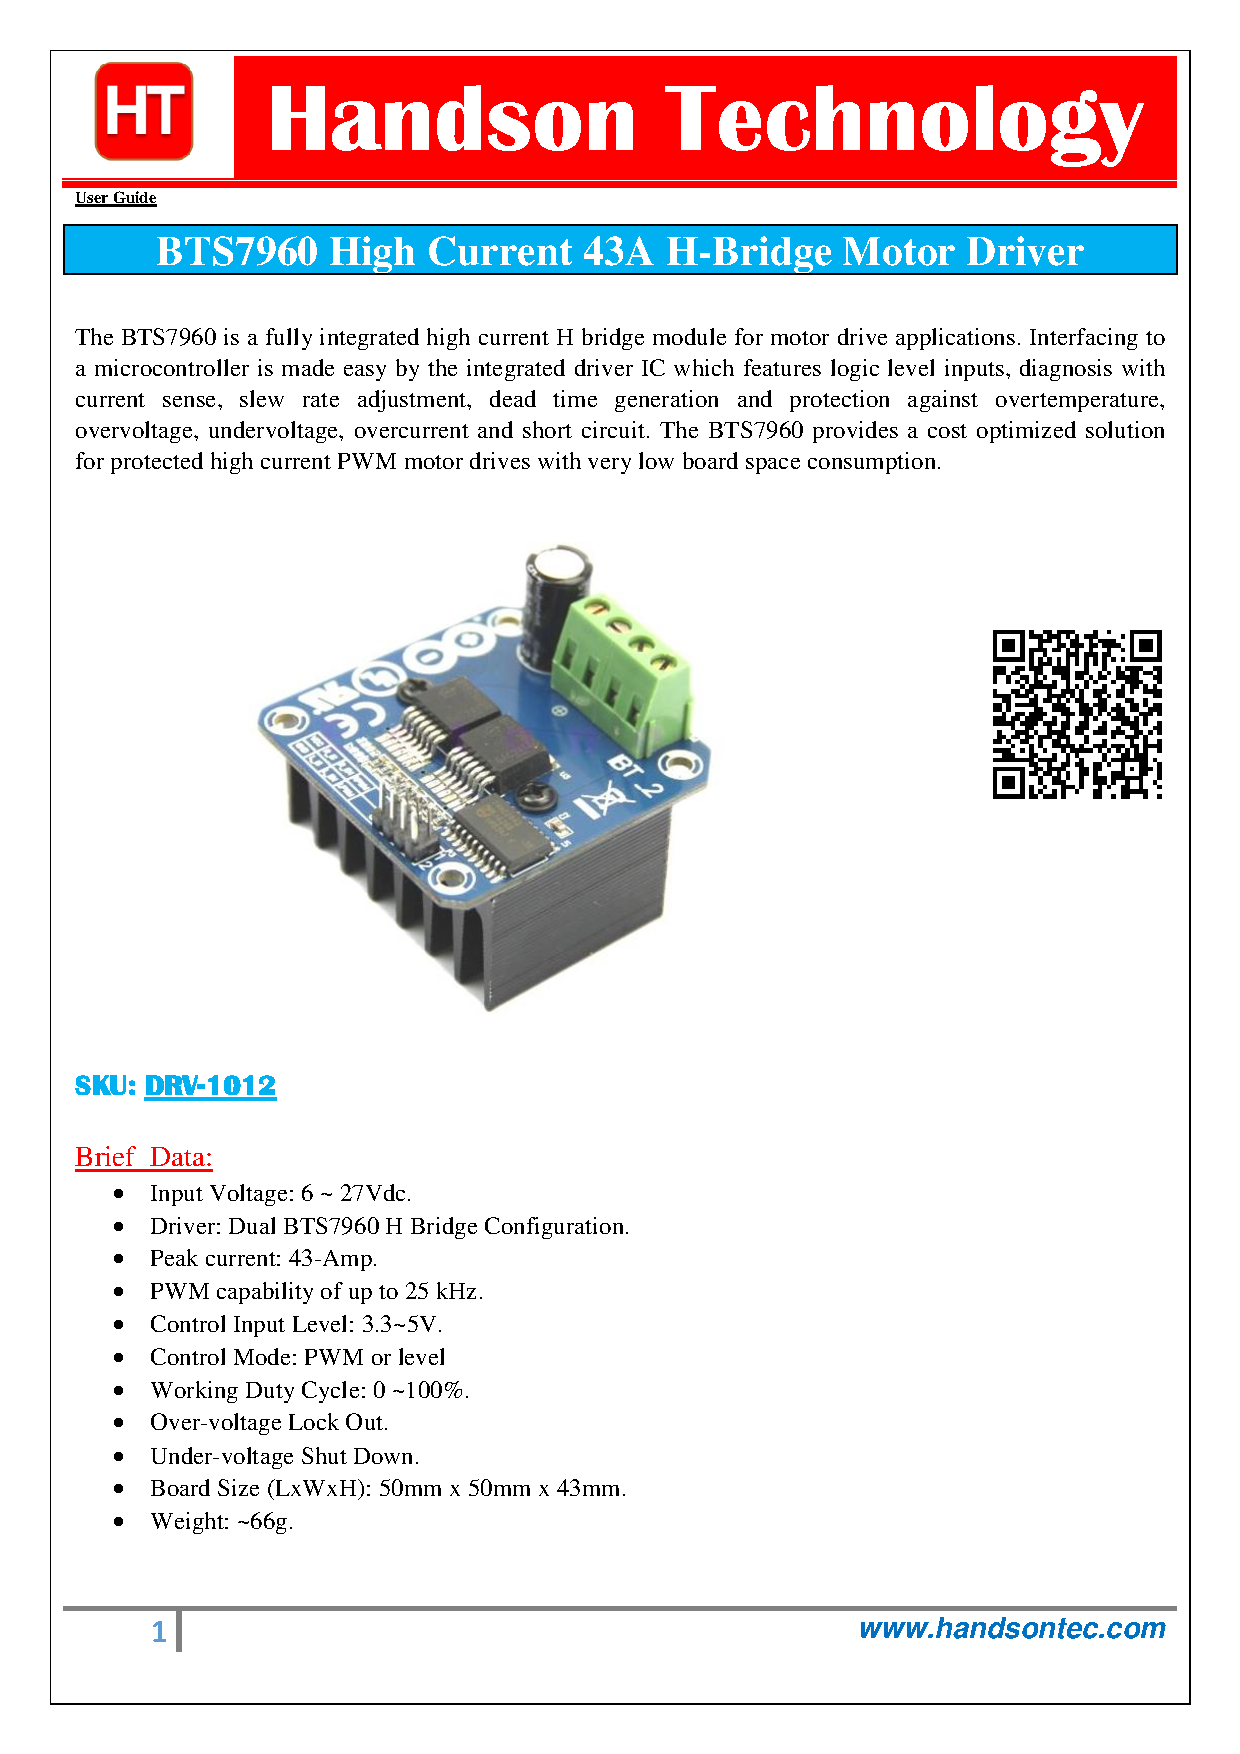
\includepdf[pages={1-7}]{docs/BTS7960 Motor Driver.pdf}






%\addchap{C Details zu Laboraufbauten und Messergebnissen}
%\setcounter{chapter}{3}
%\setcounter{section}{0}
%\setcounter{table}{0}
%\setcounter{figure}{0}
%
%\section{Versuchsanordnung}
%
%\section{Liste der verwendeten Messgeräte}
%
%\section{Übersicht der Messergebnisse}
%
%\section{Schaltplan und Bild der Prototypenplatine}
%
%\addchap{D Zusatzinformationen zu verwendeter Software}
%\setcounter{chapter}{4}
%\setcounter{section}{0}
%\setcounter{table}{0}
%\setcounter{figure}{0}

%\section{Struktogramm des Programmentwurfs}
%
%\section{Wichtige Teile des Quellcodes}
%
%\addchap{E Datenblätter}
%\setcounter{chapter}{5}
%\setcounter{section}{0}
%\setcounter{table}{0}
%\setcounter{figure}{0}
%
%%\section{Einbinden von PDF-Seiten aus anderen Dokumenten}
%
%Auf den folgenden Seiten wird eine Möglichkeit gezeigt, wie aus einem anderen PDF-Dokument komplette Seiten übernommen werden können, z.~B. zum Einbindungen von Datenblättern. Der Nachteil dieser Methode besteht darin, dass sämtliche Formateinstellungen (Kopfzeilen, Seitenzahlen, Ränder, etc.) auf diesen Seiten nicht angezeigt werden. Die Methode wird deshalb eher selten gewählt. Immerhin sorgt das Package \textit{\glqq pdfpages\grqq}~für eine korrekte Seitenzahleinstellung auf den im Anschluss folgenden \glqq nativen\grqq~\LaTeX-Seiten.
%
%Eine bessere Alternative ist, einzelne Seiten mit \textit{\glqq$\backslash$includegraphics\grqq}~einzubinden.
%
%
\includepdf[pages={2-4}]{docs/EingebundenesPDF.pdf}
%
%\clearpage
